\documentclass[a4paper,11pt]{article}
\usepackage[utf8]{inputenc} % un package
\usepackage[francais]{babel} %active le mode francais
\usepackage[top=2cm , bottom=2cm , left=2cm , right=2cm]{geometry} %propriétés de notre page
\usepackage{amsmath} %liste de symboles et applications mathématiques
\usepackage{color} %Permet d'utiliser la couleur dans nos documents
\usepackage{listings} %Paquet de coloration syntaxique (langages)
\usepackage{hyperref} % Créer des liens et des signets 
\usepackage[babel=true]{csquotes} %permet les quotations (guillemets)
\usepackage{graphicx} %Importation d'image
\lstset{language=C}
% Informations du rapport
\title {Rapport \\ Travaux Pratiques Étude des Algorithmes \\ Évaluation dynamique de programme}
\author {Quentin Tonneau - Adrien Lardenois}
\date{}
%Propriétés des liens
\hypersetup{
colorlinks=true, %colorise les liens  
urlcolor= blue, %couleur des hyperliens 
linkcolor= blue,%couleur des liens internes 
} 

\begin{document}
	\maketitle %insère l'en-tête du rapport
	\tableofcontents %insère la table des matières ATTENTION : Compiler deux fois en cas de changements
	\newpage % Nouvelle page
	
	
	\section{Introduction}
	Le but de ce projet est de fournir un logiciel capable de donner et d'évaluer le graphe de contrôle d'un programme écrit dans un pseudo langage ``simple''. Pour cela on met en place une interface très simple : on affiche un menu à choix multiple numéroté, le numéro choisi par l'utilisateur passe dans un ``switch'' qui exécute les différentes actions correspondantes. On utilise un flag pour vérifier qu'un fichier est bien en cours d'analyse pour éviter les erreurs.
	\subsection{Structures choisies}
	Pour la création du graphe en lui-même, nous avons  choisi une liste chaînée. Chaque cellule contient :
	\begin{itemize}
		\item un sommet numéroté
		\item une étiquette (qui peut être vide)
		\item la liste chaînée des arêtes qui partent de ce sommet
		\item le lien vers la cellule suivante
	\end{itemize}
	Une cellule d'arête contient : 
	\begin{itemize}
		\item le numéro du sommet d'arrivée 
		\item une étiquette (normalement l'instruction permettant de passer par l'arête)
		\item la cellule arête suivante
	\end{itemize}
	
	L'utilisation d'une liste chaînée de liste chaînée permet de simplifier la manipulation de la mémoire tout en gardant une forte cohérence des données, chaque liste d'arêtes étant attachée à son sommet d'origine. On dispose de fonctions pour ajouter des sommets et des arêtes, rechercher un sommet dans la liste, et enfin une fonction d'affichage du graphe.
	\subsection{Les fonctions d'ajout}
		L'ajout d'un sommet prend simplement le numéro et l'étiquette du sommet à créer ainsi que la liste à laquelle l'ajouter. On crée alors une nouvelle cellule et on l'ajoute en fin de liste, sauf pour une liste vide où elle devient la seule et unique cellule de la liste. En effet, l'utilisation par notre programme fait que jamais on ne créera deux sommets de même numéro et que les sommets sont créés en suivant une incrémentation régulière. Ainsi la liste proposera les sommets dans l'ordre de numérotation\footnote{qui pourra être différent de l'ordre d'exécution, surtout dans les programmes contenant des conditionnelles.}

		L'ajout d'une arête passe par une fonction intermédiaire. En apparence, on appelle \textbf{ajouter\_arête} avec pour arguments l'étiquette, le sommet de départ, le sommet d'arrivée et la liste de sommets. En fait, cette fonction n'est qu'un ``masque'' qui appelle \textbf{ajouter\_arête\_l} avec comme arguments : 
		\begin{itemize}
			\item l'étiquette
			\item la cellule du sommet de départ, donnée par \textit{recherche\_sommet(sommet\_d, liste)}
			\item le sommet d'arrivée
		\end{itemize}
		L'ajout se fait ensuite de façon standard, on crée une nouvelle cellule arête et on l'ajoute en tête de la liste d'arête.
	\subsection{Les fonctions de recherche et d'affichage}
		\label{parcourir}Ces deux fonctions reposent sur le même principe, on crée un clone de la liste que l'on parcourt ensuite.

 Dans le cas de la recherche, on s'arrête dès que l'on trouve le sommet recherché ou que l'on est arrivé à la fin de la liste. Si on a effectivement trouvé on renvoie la cellule du sommet, sinon on ajoute le sommet à la liste et on rappelle la fonction à nouveau. Une utilisation normale n'appellera jamais de sommet inconnu mais nous avons fais ce choix afin d'éviter un blocage du programme en cas d'erreur.

	Dans le cas de l'affichage, le parcours se fait systématiquement jusqu'à la fin. Pour chaque sommet, on affiche sont numéro et son étiquette, puis on parcourt sa liste d'arête de la même manière que la liste de sommet. A chaque arête, on affiche l'étiquette et le sommet d'arrivée, puis on passe à l'arête suivante. Quand la liste est finie, on passe au sommet suivant.

	\section{Ouverture et parsing}
		\textit{On considère dans la suite de ce rapport que le fichier d'entrée contient uniquement le programme, syntaxiquement correct.}
		
		Le code d'ouverture et de parsing du fichier se trouve dans les fichiers ``parser.c'' et ``parser.h''.
		\subsection{Ouverture du fichier}
		Le code permettant la lecture du fichier est simple, et commun à la plupart des applications réalisées en C. On note au passage que l'ouverture se fait en mode ``lecture'' uniquement.
		\begin{lstlisting}
FILE* fichier=NULL;
fichier=fopen(nomfichier,"r");
if(fichier==NULL)
{
	return 0; //on quitte le programme avec une erreur
}
		\end{lstlisting}
		\subsection{Parsing du fichier}
		L'algorithme repose sur une série de variables définies de la façon suivante :
		\begin{itemize}
		\item motlut : variable contenant le mot en cour de traitement (max. 50 caractères)
		\item instruction : concaténation des mots lus jusqu'à ``;''
		\item sommetactuel : numéro du dernier sommet créé
		\item nbsommet : nombre de sommet jusqu'à présent créés
		\end{itemize}
		Le parsing s'effectue à l'aide de la fonction fscanf, qui récupère un à un les mots contenus dans le fichier.
		\subsubsection{Cas général}
		Dans un fonctionnement général, c'est à dire un enchaînement d'instructions sans conditionnelle, l'algorithme concatène les mots lus jusqu'au symbole ';', puis crée une arête à l'aide de \\\textbf{ajouter\_sommet(nbsommet+1,graphe,"")} (sommet d'arrivée) puis \\\textbf{ajouter\_arête(instruction,sommetactuel,nbsommet,graphe)} dans laquelle nbsommet correspond au numéro du sommet tout juste créé.
		\subsubsection{Traitement des conditionnelles}
		Lorsque le programme rencontre le mot \textbf{Si}, il concatène l'ensemble des informations suivantes jusqu'au mot \textbf{Alors} dans une variable, crée un sommet portant pour étiquette la chaîne précédemment générée, et le relie au graphique à l'aide d'une branche vierge.
		
		Il est important de décrire la manière dont les conditionnelles sont traitées :\\
		L'algorithme possède un tableau d'entiers dans lequel on peut placer un numéro de sommet dont on nécessite de conserver sa place. Lorsque l'on rencontre un ``Si'' ou un ``Tantque'', on sauvegarde le sommet de condition dans la première case vide du tableau, et l'on crée la branche \textit{vraie}. Lorsque l'on rencontre un ``Sinon'', on remonte au sommet de conditionnelle, on stocke à la place le sommet de fin de branche gauche, et on entame la poursuite du chemin droit. Arrivé à un ``Fsi'', on crée un chemin depuis l'emplacement sauvegardé vers un nouveau sommet, un autre chemin depuis notre emplacement vers ce même sommet, et on continue le parsing. La gestion du Tantque est similaire, à l'inversion près des flèches (arrivé au Ftantque)(on revient vers le sommet sauvegardé et non le sommet créé).\\
		 La figure~\ref{image_cond} montre comment sont traitées les conditionnelles :
		\begin{figure}[!ht]\begin{center}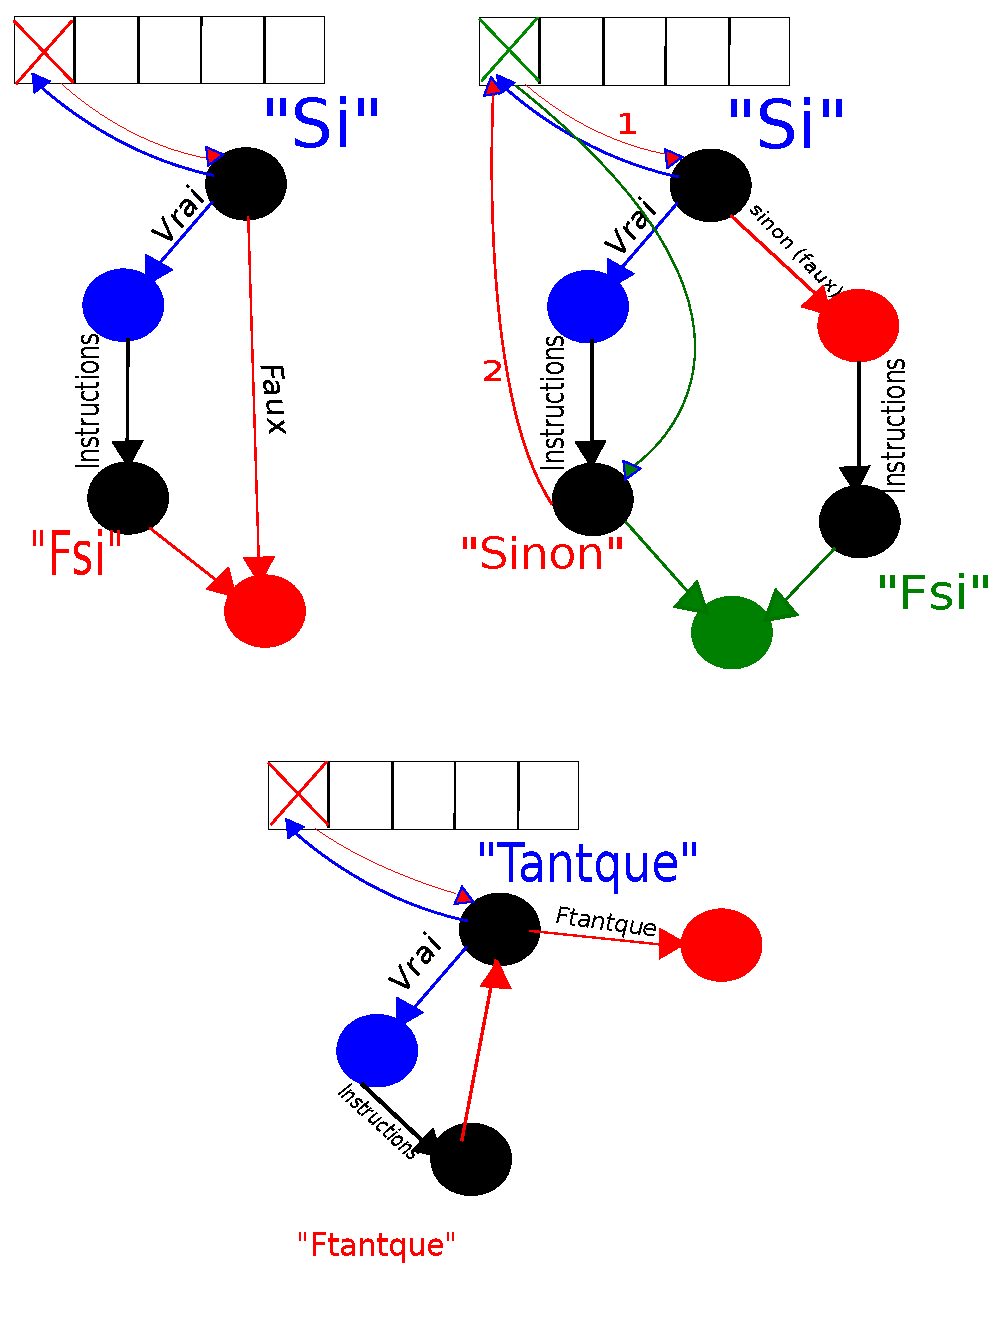
\includegraphics[width=17cm,height=7cm]{dessin.pdf}\caption{Illustration du traitement des conditionnelles}\label{image_cond}\end{center}\end{figure}
	On remarque que quelque soit le type de conditionnelle, on utilise toujours une seule case de notre \textit{Tableau de sauvegarde}. En cas d'imbrication de conditionnelles, le programme utilisera les cases suivantes, et les détruiras à la fin des traitements. Ainsi, en limitant à 50 la taille de notre tableau, nous limitons le nombre d'imbrication \textbf{maximum} à 50, ce qui est déjà une limite très grande. Un simple jeu de ré-allocation permettrait en outre de fournir une limite quasi infinie.
	\section{Analyse du graphe}
	\subsection{Mesure de McCabe}
		On utilise 2 compteurs, un pour les sommets un pour les arcs. On parcourt l'ensemble du graphe comme vu en \ref{parcourir} , mais cette fois on incrémente le compteur de sommet pour chaque cellule\_sommet et celui des arcs pour chaque cellule\_arête. En fin de graphe, on calcule et on retourne la mesure de McCabe $= Nb_{Aretes} - Nb_{Sommets} + 2$.
	\subsection{Couverture des chemins}
		La couverture des chemins prend un graphe , le chemin à remplir, la taille du chemin au moment de l'appel, la taille maximale du tableau dans lequel est gardé le chemin, et le prochain sommet à analyser. Au premier appel, le chemin donné sera vide donc de taille 0 et le prochain sommet sera le tout premier, mais lors d'appels récursifs on sera amené à fournir des chemins déjà partiellement remplis.

		La fonction parcourt le graphe, pour chaque cellule sommet on teste :
	\begin{itemize}
	\item Si la cellule suivante est NULL, on arrive à la fin d'un chemin
		\begin{itemize}
		\item on ajoute le sommet au chemin
		\item on crée une liste de chemin vide
		\item on ajoute le chemin à la liste
		\end{itemize}
	\item Sinon si la cellule a plus d'une arête dans sa liste, on est sur une conditionnelle : on vérifie si le sommet appartient déjà au chemin
			\begin{itemize}
			\item si oui, on a une boucle, donc un tant que par lequel nous sommes déjà passés
				\begin{itemize}
				\item on ajoute le sommet au chemin
				\item on saute au sommet de la première arête pour sortir du Tantque\footnote{En effet, L'ajout en tête des nouveaux arcs au moment du parsing fait que l'arête de sortie de la boucle est la première dans la liste.}
				\end{itemize}
			\item sinon, nous avons une conditionnelle traversée pour la première fois :
				\begin{itemize}
				\item on duplique la liste résultat
				\item on ajoute le sommet
				\item on duplique le chemin
				\item on défini les listes de chemins par l'appel récursif de la fonction pour le chemin déjà rempli avec comme suivant :
					\begin{itemize}
					\item le point d'arrivé du premier arc
					\item le point d'arrivé de l'arc suivant\footnote{Étant donné la structure des programmes il ne peut pas y avoir plus de 2 arcs.}
					\end{itemize}
				\item on ajoute la seconde liste à la fin de la première liste afin de regrouper tous les chemins
				\end{itemize}
			\end{itemize}
		\item Sinon on est sur un chemin simple :
			\begin{itemize}
			\item on ajoute le sommet au chemin
			\item on saute au sommet correspondant à l'arrivée de l'arête
			\end{itemize}
		\end{itemize}
		\subsection{Couverture des sommets}
			La Couverture des sommets fonctionne sur le même principe que la couverture des chemins, à la différence que lorsque l'on rencontre une conditionnelle, on vérifie son étiquette. En effet les Tantque et les Si ne sont pas traités de la même façon.

			Dans le cas d'un Tantque, on cherche d'abord tous les chemins possible dans la boucle, on les concatène et enfin on poursuit dans l'autre branche. En effet, pour la couverture des sommets on ne cherche pas tous les chemins possibles mais les chemins nécessaires pour couvrir la totalité des sommets. On cherche donc les chemins les plus longs possibles.

			Dans le cas d'un Si, si il n'y a pas de sinon, on ignore la branche faux car elle n'apporte aucun sommets. Si il y a un Sinon on crée 2 branches.
		\subsection{Couverture des arêtes}
			La couverture des arêtes fonctionne exactement comme la couverture des sommets, à ceci près que l'on ignore pas la branche faux du si car elle apporte bien un arc au graphe.
		\subsection{Affichage des couvertures}
			L'affichage se fait par un simple parcours de la liste, avec un affichage de chaque case du chemin de la cellule.
	\section{Pour aller plus loin}
	Il nous était demandé également de réaliser un algorithme de génération de jeux de test. N'ayant pas une définition exacte de la syntaxe et des possibilités du langage de programmation, il nous est impossible de réellement générer des jeux de test sous la forme $\{x=4,y=\frac{6}{3}\}, $. Nous avons donc pensé prendre les étiquettes de chacune de nos conditionnelles dans le cadre de la couverture des instructions, et les relier par un symbole \textbf{\&}. Ensuite, la négation de ces expressions aurait pu nous donner une couverture complète du programme par jeux de test. Par exemple $\{a<3\ \&\ a>c\ \&\ c=2\}$. Cette solution, facile à mettre en place, possède malheureusement des lacunes :
	\begin{itemize}
	\item Impossible de vérifier les incohérences dans les conditionnelles ($a<b$ et $b<a$)
	\item Difficultés à réaliser les inverses de ces expressions (traitement du langage)
	\item Impossibilité de traiter les boucles Tantque, car les variables changent au cours du parcours, et la variable d'entrée est l'inverse de celle de sortie
	\end{itemize}
	Devant le grand nombre de problèmes issue d'un tel processus, nous n'avons pas souhaité créer l'algorithme associé.
	
	Nous aurions pu également afficher la liste des programmes présents dans le répertoire d'exécution et proposer à l'utilisateur d'en choisir un, mais tout comme l'organisation d'un projet, les sources sont généralement réparties dans différents répertoires, aussi il est plus simple de rentrer le chemin du fichier au clavier.

	Pour pouvoir générer des jeux de tests, la plupart des variables étant amenées à changer au cours du programme,  il serait nécessaire d'implémenter un système de backtracking pour vérifier que les jeux de test permettront la complétion du programme.
	\section{Conclusion}
		Ce projet nous a permis de mettre en pratique les connaissances acquises en début de semestre (graphes et couvertures), d'approfondir notre maîtrise des listes chainées, fonctions récursives, allocation dynamique en C. Nous regrettons de n'avoir pu utiliser le langage C++, notamment dans la gestion des chaînes de caractères et des structures (programmation orientée objet).
		


L'ensemble du projet est fonctionnel sous l'environnement suivant : Ubuntu 11.10 X64 et gcc v.4.6.1. La plupart des programmes ne fonctionnent pas sur les ordinateurs de la faculté, probablement par manque de mémoire vive et système d'exploitation équivalent.
		
	Finalement nous avons pu fournir un programme globalement fonctionnel, mais il nous aurai fallu plus de temps pour pouvoir mettre en place les couvertures et jeux de tests manquants.

		
\end{document}
